\documentclass[aps,prl,reprint]{revtex4-1}
\usepackage{blindtext}

\usepackage{amsmath}
\usepackage{graphicx}
\usepackage{commath}
\usepackage{siunitx}
\usepackage{tabularx}
\usepackage{subcaption}

\usepackage{amssymb}

\usepackage{float}

\usepackage{graphicx}


\usepackage[b]{esvect}

\newcommand{\de}{\mathrm{d}}
\newcommand{\vcc}{V_\text{cc}}
\newcommand{\parallelsum}{\mathbin{\!/\mkern-5mu/\!}}

\graphicspath{ {images/} }
\begin{document}
\title{Unit 4: Transistors and Transistor Circuits}
\author{Xueqi Li}
% \email{xueqi.li@stonybrook.edu}
\thanks{Partner: Tianming Hai}
% \author{partner Tianming Hai}
\noaffiliation
\date{Mar 24, 2018}


% \begin{abstract}
% Here I tell what I have done... And I have done a lot but it is hard to tell what exactly I have done...
% \end{abstract}

\maketitle

\section{Introduction}  
There are a few importent applications for the semiconductor, one of the most importent one is transistors. In this lab report, bipolar junction transistor (BJT) and junction gate field-effect transistor (JFET) will be introduced.

\subsection{Bipolar Junction Transistor}
A bipolar junction transistor transistor is made by p-type and n-type semiconductor. For example, one can form a transistor by putting p-type semiconductor in between of two n-type semiconductor. Such transistor will form a p-n junction at the interface, which lead to potential. We call the connection to the middle p-typle as base, call the connections to the two n-tpye as collector and emiter. Easy to see that if there is current flowing from base to emiter, the voltage drop between the base and the emiter is the voltage drop due to a p-n junction:
\begin{equation}
    V_{B\!E} = V_d \label{eq:Vbd}
\end{equation}
where $V_d$ is usually 0.65V.

If there is nothing connect to the base, or the voltage applied on base is less than $V_d$, which is not enough to break the potential of the p-n junction, the transistor is simply two diode face each other, which means on current can flow through the transistor from collector to emiter or vice versa.

If there is some voltage applied on the base and higher than $V_d$. This will allow the current to folw through the transistor. If there is a voltage $V_C$ applied on collector, than the current will flow to the emiter. Moreover, more voltage applied to the base, the transistor will allow more current to flow. It turn out that it is a linear relation in the most of the case:
\begin{equation}
    I_C = \beta I_B \label{eq:ic}
\end{equation}
where $\beta$ is different from different transistor. its value is usually around 50-300.

Furthermore, one can also apply Kirchhoff's circuit laws:
\begin{equation}
    I_C + I_B = I_E \label{eq:kirchhoff}
\end{equation}
than it is possible to use Equation~\ref{eq:ic} to find the current in emiter:
\begin{equation}
    I_E = (1 + \beta)I_B \label{eq:ie}
\end{equation}

So as above, one can also find following relation:
\begin{equation*}
    I_C = \alpha I_E \ ; \  \alpha = \frac{\beta}{1 + \beta} \approx 1
\end{equation*}

One must see that the output voltage cannot larger then the voltage input (base voltage and collector volrage) to the transistor. If $\vcc$ is applied in at somewhere connect to the collector, usually we have following relation:
\begin{equation}
    \vcc > V_C > V_B > V_E \ge 0 \label{eq:vle}
\end{equation}

Usually a transistor have a maximum power so that it would not be broken. Thus we have
\begin{equation*}
    P = I_C V_{C\!E} \le P_\text{max}
\end{equation*}
which is used to protect the transistor

Overall, such a transistor is like a valve. The base control the valve to open or close (or open in some percentage) the gate between the collector and the emiter. Moreover, if all the input in the collector is already go through the transistor to the emiter, no matter how much force is putting in in to the valve, the output would not change.

\subsection{Emitter Follower}
\begin{figure}[h]
    \centering
    \includegraphics[height=1.4in]{image/Follower.pdf}
    \caption{A Emitter Follower}
    \label{fig:follower}
\end{figure}
An emitter follower is an application of the bipolar junction transistor, which is presented as Figure~\ref{fig:follower}. From Equation~\ref{eq:Vbd} we can easy to see that the output voltage is simply given by
\begin{equation}
    V_\text{out} = V_\text{in} - V_d \label{eq:follower}
\end{equation}

One importent aspect for the follower is that it isolation the circuit like a buffer, i.e., it have a low influence on the input side. and it also makes the circuit functioning well on the output side. This means the it have a high input impedance and a low output impedance.

The output impedance is to think the circuit as its Thevenin's equivalent. Than we have:
\begin{equation*}
    Z_\text{out} = \frac{\de V_\text{open}}{\de I_\text{short}} = 0 
\end{equation*}

The input impedance is defined as $\frac{\de V_\text{in}}{\de I_\text{in}}$. Thus, we have:
\begin{equation*}
    Z_\text{in} = \frac{\de V_\text{in}}{\de V_\text{in}} = \frac{\de V_B}{\de \frac{V_B - V_d}{(1+\beta)R_E}} = (1+\beta)R_E
\end{equation*}
which is usually very large since $\beta$ is from 50 to 300.

\subsubsection{Emitter Follower Application}
\begin{figure}[h]
    \centering
    \includegraphics[height=1.2in]{image/Follower-Full.pdf}
    \caption{A Emitter Follower in Application}
    \label{fig:followerFull}
\end{figure}

In practice, we use a emitter follower as presented in Figure~\ref{fig:followerFull}. The reasone that we cannot use a circuit as Figure~\ref{fig:follower} is because of Equation~\ref{eq:vle}. Let say if we have a sine wave centered at 0V from the input, than any part below 0V will be cut by Equation~\ref{eq:vle}. So as any part larger than around $\vcc$. Therefore, by using a circuit as Figure~\ref{fig:followerFull}, we can centered the comming wave in the acceptable range, i.e., approximately (voltage might drop due to p-n junction) from 0V to $\vcc$. Thus we want to center the output voltage such that $V_E \approx \frac{\vcc}{2}$

To decide the value of different part of the circuit, we can simply follow the follow procedure:
\begin{enumerate}
    \item Set $V_E = \frac{\vcc}{2}$ when input voltage is zero. This will center the output voltage.

    \item Set $R_E$ to limit the maximum current ($I_E$) by 
    \[
    R_E = \frac{V_E}{I_E(\text{max})}
    \]

    \item Set $R_1$ and $R_2$ to achieve our setting of $V_E$. To do so we find 
    \[
    V_B = V_E + V_d = \frac{\vcc R_2}{R_1 + R_2}
    \]
    Also, we want to have $Z_\text{EF:in}\gg R_\text{VD:th}$. To do so let say $Z_\text{EF:in}$ is around $\beta$ times larger than $R_\text{VD:th}$. Than we can have 
    \[
    \frac{R_1R_2}{R1+R_2} \approx R_E
    \]
    Using above two equation we can therefore solve $R_1$ and $R_2$.

    \item Set $C$ by expected frequency. This step we think the circuit as a high-pass. Thus, we have 
    \[
    C = \frac{1}{2\pi f R} = \frac{1}{2\pi f (R_1 \parallelsum R_2 \parallelsum Z_\text{in})}
    \]
\end{enumerate}

\subsection{Common Emitter Amplifier}
\begin{figure}[h]
    \centering
    \includegraphics[height=1.3in]{image/Common-Emitter-Amplifier.pdf}
    \caption{A Common Emitter Amplifier}
    \label{fig:amplifier}
\end{figure}
Another application of bipolar junction transistor is the common emitter amplifier presented in Figure~\ref{fig:amplifier}. We see that the output voltage can be find by using Equation~\ref{eq:kirchhoff}, Equation~\ref{eq:ic} and Equation~\ref{eq:ie}
\begin{align*}
    V_\text{out} &= V_C \\
                 &= \vcc -I_CR_C \\
                 &= \vcc -\alpha I_E R_C\\
                 &= \vcc - \alpha \frac{V_\text{in} - V_d}{R_E}R_C
\end{align*}

One can calculate teh gain of the circuit as:
\begin{equation*}
    \text{Gain}:=\frac{\de V_\text{our}}{\de V_\text{in}} = -\alpha\frac{R_C}{R_E} \approx -\frac{R_C}{R_E}
\end{equation*}
where the negative sign imply that the output will be inverse from the input. From thi we can see that by choosing $R_C$ and $R_E$, we can amplify the signal.

One can also calculate the input impedance as:
\[
Z_\text{in} = \frac{\de V_\text{in}}{I_\text{in}}=\frac{\de V_\text{in}}{\de \frac{V_\text{in} - V_d}{(1+\beta)R_E}} = (1+\beta)R_E
\]

To find the output impedance, consider we use a load resistor in the output end and measure the voltage on the load resistor:
\begin{align*}
    V &= V_C\\
      &=I_LR_L \\
      &= (I_\text{cc} - I_C)R_L\\
      &= (\frac{\vcc-V}{R_C}-\beta I_E)R_L\\
      &= (\frac{\vcc-V}{R_C}-\beta \frac{V_E}{R_E})R_L \\
      &= (\frac{\vcc-V}{R_C}-\beta \frac{V_\text{in} - V_d}{R_E})R_L
\end{align*}
sove for $V$, we find
\[
V = \frac{R_L}{R_C+R_L} \vcc - \frac{R_CR_L}{R_C+R_L}\frac{\alpha (V_\text{in}-V_d)}{R_E}
\]
Now we can find output impedance by using voltage divider equation:
\begin{align*}
    Z_\text{out} = R_\text{th} &= \frac{V_\text{th} R_L}{V} - R_L \\
                               &= \frac{(\vcc - \alpha \frac{V_\text{in} - V_d}{R_E}R_C) R_L}{\frac{R_L}{R_C+R_L} \vcc - \frac{R_CR_L}{R_C+R_L}\frac{\alpha (V_\text{in}-V_d)}{R_E}} - R_L\\
                               &= \frac{\vcc - \alpha \frac{V_\text{in} - V_d}{R_E}R_C}{\frac{1}{R_C+R_L} \vcc - \frac{R_C}{R_C+R_L}\frac{\alpha (V_\text{in}-V_d)}{R_E}}- R_L\\
                               &= \frac{\vcc - \alpha \frac{V_\text{in} - V_d}{R_E}R_C}{\frac{1}{R_C+R_L} (\vcc - R_C\frac{\alpha (V_\text{in}-V_d)}{R_E})}- R_L\\
                               &=R_C + R_L - R_L\\
                               &=R_C
\end{align*}
which we can find out the output impedance is $R_C$.

\subsubsection{Common Emitter Amplifier Application}
\begin{figure}[h]
    \centering
    \includegraphics[height=1.3in]{image/Common-Emitter-Amplifier-Full.pdf}
    \caption{A Common Emitter Amplifier in Application}
    \label{fig:amplifierFull}
\end{figure}
Due to the same reason as the follower, in practice, we use a circuit as presented in Figure~\ref{fig:amplifierFull}. This will center the output voltage in the position we want within the limit of Equation~\ref{eq:vle}. To find the value for each part of the circuit, we can following the same steps as follower case with a small change:
\begin{enumerate}
    \item Set voltage for bace, emiter and collector. If the input have amplitude $A$, than the range for them are given as
    \begin{align*}
        V_B &= V_d \sim V_d + V_E(\text{max}) \\
        V_E &= 0 \sim 2A \\
        V_C &= V_B(\text{max}) \sim \vcc
    \end{align*}
    which lead to following quiessent voltage:
    \begin{align*}
        V_B &= V_E(0) + V_d \\
        V_E &= A \\
        V_C &= \frac{\vcc + V_d + 2 A}{2}
    \end{align*}
    \item Set $R_E$ to limit the current:
    \[
    \frac{V_E(\text{max})}{R_E} = I_\text{limit}
    \]
    \item Set $R_C$ for the given gain:
    \[
    \frac{R_C}{R_E} = \text{Gain}
    \]
    \item Set $R_1$ and $R_2$ to achieve $V_B$, here we do the same trick as follower:
    \begin{align*}
        V_B = \frac{\vcc R_2}{R_1 + R_2}\\
        \frac{R_1R_2}{R_1 + R_2} = R_E
    \end{align*}
    \item Set $C$:
    \[
    C = \frac{1}{2\pi f (R_1 \parallelsum R_2 \parallelsum Z_\text{in})}
    \]
\end{enumerate}

\subsection{Field-effect Transistor}
\begin{figure}[h]
    \centering
    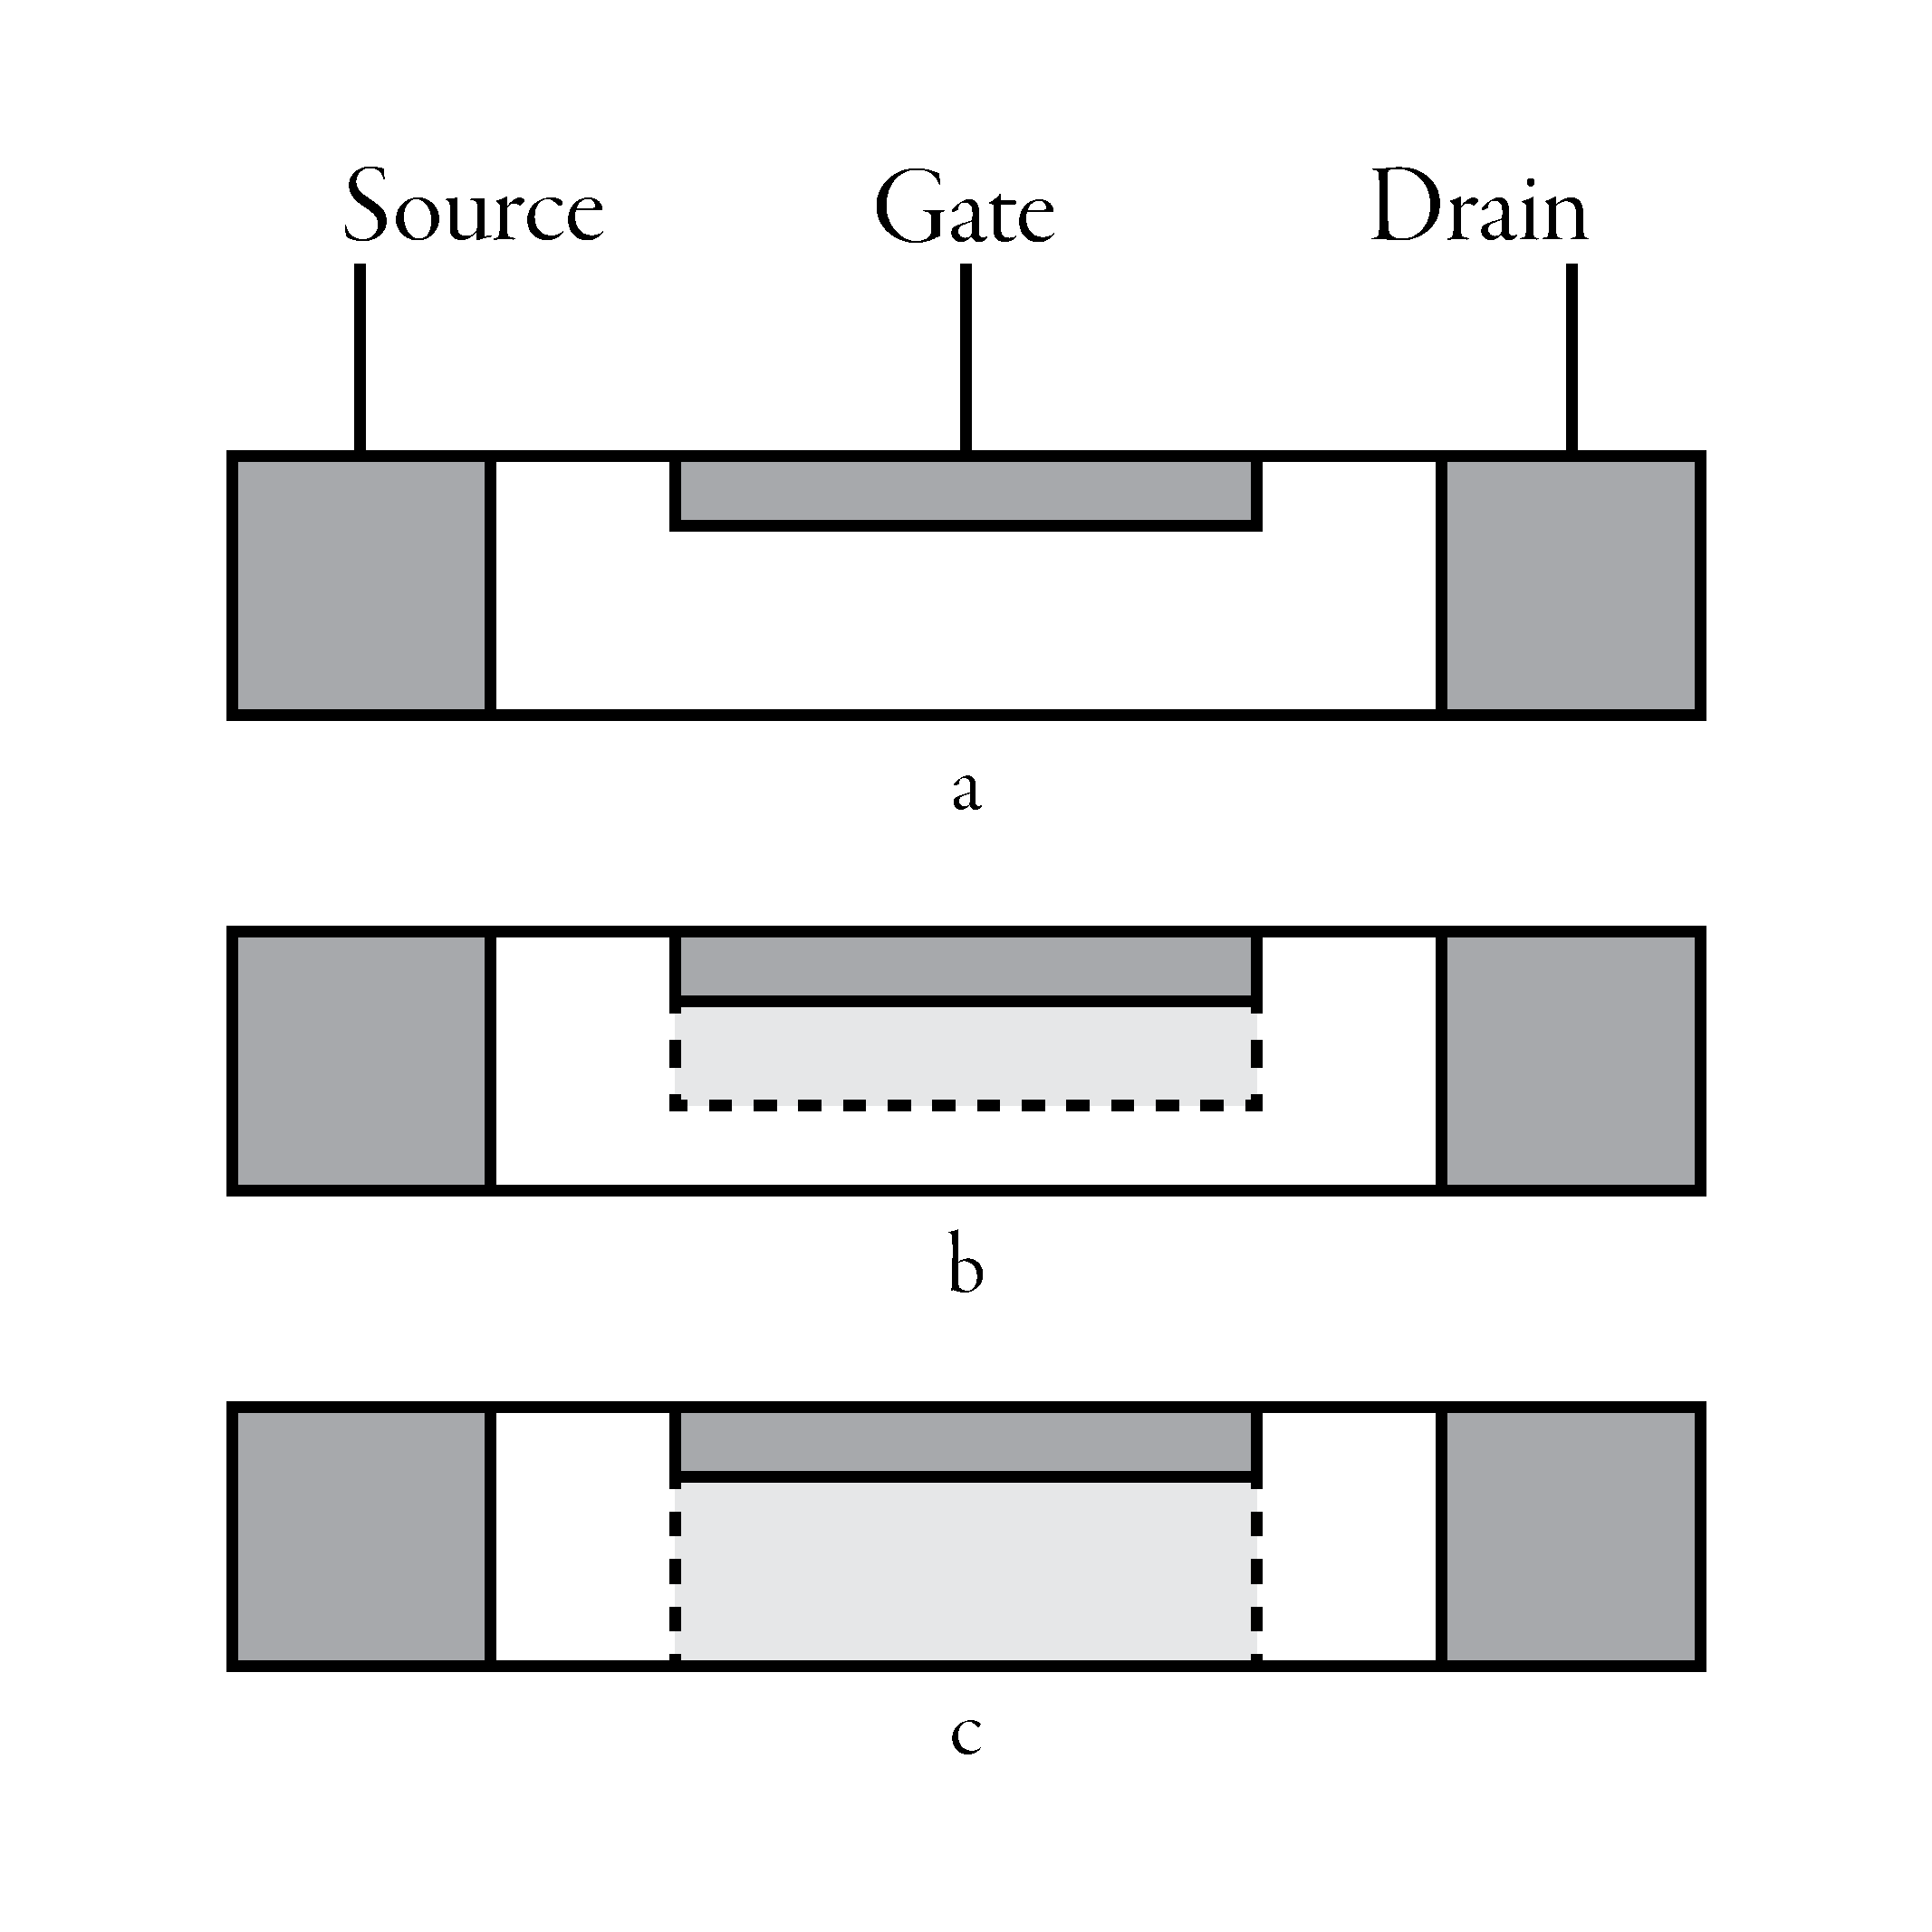
\includegraphics[height=2in]{image/JFET.pdf}
    \caption{Junction Field-effect Transistor}
    \label{fig:jfet}
\end{figure}
Another transistor is the field effect transistor. The structure of a JFET is present in Figure~\ref{fig:jfet}a. The dark gray part is p-type semiconductor and the white part is n-type semiconductor.

When one apply a some voltage on the gate, a field effect will happened when $V_G < 0$. The field effect will create a light gray area as presented in Figure~\ref{fig:jfet}b. This area will prevent current to pass this area. Eventually, this aria will grow and cut the whole transistor, as present in Figure~\ref{fig:jfet}c, which let no current flow through. Such voltage so called as pinch-off voltage. After that voltage, it stays as a open circuit.

\section{Data and Calculation}
\subsection{Bipolar Junction Transistor}
\begin{figure}[h]
    \centering
    \includegraphics[height=1in]{image/Measure-BJT.pdf}
    \caption{Measure BJT}
    \label{fig:bjtLab}
\end{figure}
In here we use Figure~\ref{fig:bjtLab} to measure the property of a BJT. To avoid damage the BJT, we want to limit the input current. Notice the voltage accros $R_0$ and $R_2$ are $5V - V_d$, where we take $V_d$ as 0.65V. By using Equation~\ref{eq:ic}, we chose to use a 3.39(1)k$\Omega$ resistor. The data obtained in is list in the appendix.

\subsection{Follower}
\begin{figure}[h]
    \centering
    \includegraphics[height=1.2in]{image/Follower-Full-Lab.pdf}
    \caption{Follower in Lab}
    \label{fig:followerLab}
\end{figure}
We follow the step above to find the value of each part of circuit.
\begin{enumerate}
    \item Set $V_E = \frac{\vcc}{2} = 7.5V$ when input voltage is zero.

    \item Set $R_E$ to limit the maximum current ($I_E$) by 
    \[
    R_E = \frac{V_E}{I_E(\text{max})} = \frac{7.5V}{5\text{mA}} = 1500\Omega
    \]

    \item Set $R_1$ and $R_2$ to achieve our setting of $V_E$. To do so we find 
    \begin{align*}
        V_B = V_E + V_d = 8.15V &= \frac{15V R_2}{R_1 + R_2}\\
        \frac{R_1R_2}{R1+R_2} &= 1500\Omega
    \end{align*}

    Using above two equation we can therefore solve $R_1 = 2760.74\Omega$ and $R_2=3283.67\Omega$.

    \item Set $C$ by expected frequency, here we use $f = 300$Hz. This step we think the circuit as a high-pass. Thus, we have 
    \[
    C = \frac{1}{2\pi f (R_1 \parallelsum R_2 \parallelsum Z_\text{in})} = \frac{1}{2\pi f 1496.8 \Omega}=3.5368\times 10^{-11}\mu F
    \]
    In lab we measure following value for each part:
    \begin{align*}
        R_E &= 1.54(1)\text{k}\Omega\\
        R_1 &= 2.80(1)\text{k}\Omega\\
        R_2 &= 3.15(20)\text{k}\Omega\\
        C &= 0.35(1)\mu F
    \end{align*}
    The data obtained is in the appendix.

    We also measure the DC voltage in each end of the follower, we find $V_C = 15.0(2)V$, $V_B = 8.2(2)V$, and $V_E = 8.0(2)V$.
\end{enumerate}
\subsection{Amplifier}
\begin{figure}[h]
    \centering
    \includegraphics[height=1.2in]{image/Common-Emitter-Amplifier-Full-Lab.pdf}
    \caption{Amplifier in Lab}
    \label{fig:amplifierLab}
\end{figure}
For amplifier, we follow the step above to find the value of each part of the circuit:
\begin{enumerate}
    \item Set quiessent voltage for bace, emiter and collector. 
    \begin{align*}
        V_B &= V_E(0) + V_d = 0.5 + 0.65V = 1.15V \\
        V_E &= A = 0.5V \\
        V_C &= \frac{\vcc + V_d + 2 A}{2} = \frac{15+0.65+1}{2}V=8.325V
    \end{align*}
    \item Set $R_E$ to limit the current:
    \[
    \frac{V_E(\text{max})}{R_E} = \frac{1V}{R_E}= I_\text{limit} = 0.5\text{mA}
    \]
    This give use $R_E = 2000\Omega$.
    \item Set $R_C$ for the given gain:
    \[
    \frac{R_C}{R_E} = \frac{R_C}{2000\Omega} =  \text{Gain} = 15
    \]
    This give us $R_C = 30\text{k}\Omega$.
    \item Set $R_1$ and $R_2$ to achieve $V_B$, here we do the same trick as follower:
    \begin{align*}
        V_B = 1.15V = \frac{\vcc R_2}{R_1 + R_2} &= \frac{15V R_2}{R_1 + R_2}\\
        \frac{R_1R_2}{R_1 + R_2} &= R_E = 2000\Omega
    \end{align*}
    Solve the equation we find $R_1 = 26087\Omega$ and $R_2 = 2166.06\Omega$
    \item Set $C$, here we use $f = 200$Hz:
    \[
    C = \frac{1}{2\pi f (R_1 \parallelsum R_2 \parallelsum Z_\text{in})} = 3.939\text{nF}
    \]
\end{enumerate}
    
    In the lab, we measure following value:
    \begin{align*}
        R_E &= 1.969(1)\text{k}\Omega\\
        R_C &= 29.75(3)\text{k}\Omega\\
        R_1 &= 27.02(1)\text{k}\Omega\\
        R_2 &= 2.200(5)\text{k}\Omega\\
        C &= 4.2\text{nF}
    \end{align*}

    The data obtained is as in the appendix.

\subsection{JFET}
\begin{figure}[h]
    \centering
    \includegraphics[height=2in]{image/JFET-Measure.pdf}
    \caption{Measure JFET}
    \label{fig:jfetMeasure}
\end{figure}
In this lab we use Figure~\ref{fig:jfetMeasure} to measure the property of JFET. The data obtained is in the appendix.

\section{Analysis}
\subsection{Measure BJT}
In here we measure the current in base and in collector. We change the variable resistor to obtained different current in the base. The gain is given in the Table 1. We see that gain is equal to $\beta$ and is not a constent in the whole range. The gain decrease as the current on base increase, and the current in collector stop increase once it reach $\vcc$, which follows Equation~\ref{eq:vle}.

On the other hand, we can measure the voltage drop between the emiter and the collector, which is in Table 2. We see it is not in saturation, i.e., increase current in base do make current in collector increase, untill current in collector reache $\vcc$, it than in saturation, i.e., increase current in base does not chagne the collector current. We can also see this in from the voltage. When in the saturation, we can think as the valve are full open, whicn means the voltage drop between collector and the emiter is very small. We see that before collector current reach around 16V, the voltage drop is large, which means it is not in saturation. However, when collector current is larger than around 16V, the voltage drop is small, which means it is now in saturation.

\subsection{Follower}
We see that the DC voltage between base and emiter droped 0.2V, which is reasonable, this BJT might have a smaller $V_d$. To see the effect of the follower, we can add a small load resistor in the output end and measure the voltage of it. When we have the follower, the voltage on load resistor is much larger (same as without load resistor) than the case of withouht follower, which means the follower indeed performs its main function of increasing the output impedance.

    \begin{figure*}[t]
    \centering
    \subcaptionbox{Follower $V_\text{out}/V_\text{in}$}[.49\linewidth][c]{%
        \includegraphics[width=.4\linewidth]{image/table3plot.pdf}}\quad
    \subcaptionbox{Phase of Follower}[.49\linewidth][c]{%
        \includegraphics[width=.4\linewidth]{image/phase.pdf}}
    \caption{Plot for FET}
    \label{fig:table3plot}
    \end{figure*}

We apply a 10V peak to peak input voltage to the follower, and we obtained data in Table 3. From the data, we can plot Figure~\ref{fig:table3plot}. We can also see that the phase decrease as frequency become higher linearly in log scale unhtill output voltage reachs $\vcc$. These are characteristics of a high pass. Recall, for high pass, we have
\begin{align*}
    \abs{V_R} &= 
    \begin{cases}
        V_\text{in},                & \text{if } \omega R C \gg 1;\\
        \frac{V_\text{in}}{\sqrt{2}}, & \text{if } \omega R C = 1;\\
        V_\text{in}\omega R C,      & \text{if } \omega R C \ll 1\\
    \end{cases}\\
    \varphi &= 
    \begin{cases}
        \frac{\pi}{2},                & \text{if } \omega R C \rightarrow 0;\\
        \frac{\pi}{\sqrt{4}}, & \text{if } \omega R C = 1;\\
        0,      & \text{if } \omega R C \rightarrow \infty\\
    \end{cases}\\
\end{align*}
where here $f = 300$Hz. We see that in our result, phase decrease as frequency become higher followes above equations on phase. So as the output voltage.

We also measure the output voltage with a fixed frequency 10kHz, so as in Table 4. We see that the output voltage followes the input voltage untill it reachs $\vcc$ and stays at $\vcc$ when we increase the input voltage.

One interesting thing is that the output voltage sometimes higher than the input voltage by around 0.4(2)V. That may due to some background noise voltage.

\subsection{Amplifier}
\begin{figure}[b]
    \centering
    \includegraphics[height=2in]{image/amplabpic.pdf}
    \caption{Higher than 7.5V}
    \label{fig:ampLabPic}
\end{figure}
When we build the circuit, we notice that the divider is asymmetri, while in the follower case it is almost symmetric. The reason is that in the voltage case, we chose to center the output voltage around $V_E = \frac{\vcc}{2} = V_B + V_d$. For example, we centered $V_B$ in our case as 8.15V. so that we use a almost symmetric divider by the divider equation:
\[
V_\text{B:center} = \frac{R_2 \vcc}{R_1 + R_2}
\]
However, when we build the amplifier, we do not center our quiessent voltage in $\frac{\vcc}{2}$, we center the output voltage in a much higher voltage to give space for $V_E$ and $V_B$, follows Equation~\ref{eq:vle}. Moreover, our $V_C$ have a much larger amplitude than $V_B$ and $V_E$. Thus $V_B$ and $V_E$ have to be cnetered very low. For example, in our case, we center $V_B$ at 1.15V. From the divider equation we can see we have to use a very asymmetri divider to divider the voltage to such a low voltage.

In the lab, we see that we achieve a amplitude with gain of 13. This is within the range of 15\% of 15 (12.75 to 17.25). Also we find in the lab that output is inverted compared to the input, which follows our result in Introduction. This result is successful. We test the divice with different frequency as in Table 5 (larger than 200Hz) and Table 6 (less than 200Hz). We can also see that in high frequency, there is no phase shift, follows the high-pass equation, i.e., it will not produce a phase shift in high frequency but it do produce a phase shift in low frequency. The output indeed shift by around 7.5V. If we increase the amplitude greater than 7.5V, we see that the output peak curved to follow the Equation~\ref{eq:vle}, to follow the shape of $V_B$ and any voltage higher than $\vcc$ will be cut, so as in Frgure~\ref{fig:ampLabPic}. 

To calculate transcoductance, We see
\begin{align*}
    g &= \frac{I_\text{out}}{V_\text{in}} \\
      &= \frac{I_\text{cc} + I_C}{V_\text{in}}\\
      &= \frac{\frac{\vcc + V_C}{R_C} - \alpha I_E}{V_\text{in}} \\
      &= \frac{\frac{\vcc + V_\text{out}}{R_C} - \alpha \frac{V_E}{R_E}}{V_\text{in}}\\
      &= \frac{\frac{15V + 8.325V}{30000\Omega} - \frac{1.15V - 0.65V}{2000\Omega}}{1.15V}\\
      &= 0.00041\mho
\end{align*}

\subsection{FET}

    \begin{figure*}[t!]
    \centering
    \subcaptionbox{$I_D$ v. $V_G$ on maximum $V_D$}[.3\linewidth][c]{%
        \includegraphics[width=.3\linewidth]{image/ivvg.pdf}}\quad
    \subcaptionbox{$I_D$ v. $V_D$ on $V_G = 0V$}[.3\linewidth][c]{%
        \includegraphics[width=.3\linewidth]{image/lvvdg0.pdf}}\quad
    \subcaptionbox{$I_D$ v. $V_D$ on $I_D(V_D = \text{max}) = 1mA$}[.3\linewidth][c]{%
        \includegraphics[width=.3\linewidth]{image/ivvdgn.pdf}}
    \footnotetext{Some error bar on voltage and current are too small to see}
    \caption{Plot for FET}
    \label{fig:fetPlot}
    \end{figure*}

    \begin{figure*}[t!]
    \centering
    \subcaptionbox{A close look when $V_G = 0V$}[.49\linewidth][c]{%
        \includegraphics[width=.4\linewidth]{image/fit1.pdf}}\quad
    \subcaptionbox{A close look when $I_D(V_D = \text{max}) = 1mA$}[.49\linewidth][c]{%
        \includegraphics[width=.4\linewidth]{image/fit2.pdf}}
    \footnotetext{Some error bar on voltage and current are too small to see}
    \caption{A close loof for plot for FET}
    \label{fig:fetPlotClose}
    \end{figure*}

To find the pinch-off voltage, we measure the $V_G$ and $I$ as $V_D = 10V$. The result is in Table 7. From the data we see that the pinch-off voltage is around -1.50(4)V. Which within the range of a 2N5457 transistor\cite{jfet} (-0.5V to -6V), which is used in lab. When we chose $V_G = 0$, we find that at the highes $V_D$, (Table 8) we find $I_D = 2.934(1)$mA, which is also withing the range of a 2N5457 transistor\cite{jfet} (1 to 5 mA). 

When we fixed $V_D$ at the highest voltage we can have, the measurment resutl is in Table 10. We can therefore obtained Figure~\ref{fig:fetPlot}a.

When we fixed gate voltage, we can obtained data in Table 8 and Table 9. One with gate voltage is zero, and the other one is so that gate voltage gives $I_D = 1$mA on the largest voltage on drain. At this point $V_G = -0.62(2)$V. We see that at low voltage, the relation between current and the voltage is linear, which means that the transistor behaves like a voltage dependent resistor. We can take a close look at the result of Figure~\ref{fig:fetPlotClose}. After preform a linear fit, we can find the resistor value. When $V_G = 0V$, we have $R = 421.1(50)\Omega$. And when $I_D(V_D = \text{max}) = 1mA$, we have $R = 740.7(72)\Omega$. In this case, the transconductance is just inverse resistor. Thus we find when $V_G = 0V$, we have $g = 0.00237(5)\mho$. And when $I_D(V_D = \text{max}) = 1mA$, we have $g = 0.00135(6)\mho$.
\section{Conclusion}
The result is this lab si great. The experiment result follows the theory in introduction. The only one problem is sometimes the output voltage is higher than the input voltage in the follower. That might due to a background noise voltage and $V_d$ for the the transistor used in the lab are too samll.


\bibliography{cite}
\bibliographystyle{apsrev4-1}

    % \begin{figure}[h]
    %     \centering
    %     \includegraphics{images/plot2.pdf}
    %     \caption{A voltage divider}
    %     \label{fig:2}
    % \end{figure}

    % \begin{table}[h]
    % \begin{ruledtabular}
    % \begin{tabular}{cccc} 
    % Load[k$\Omega$] &  Output Voltage[V] & $R_\text{th}[\Omega]$ & Theoretical Voltage\\ \hline\hline
    % 50              & 0.680(1)           & 501(1)                & 0.682 \\ \hline
    % 500             & 3.75(1)            & 500(1)                & 3.75 \\ \hline
    % 5000            & 6.80(1)            & 514(1)                & 6.82 \\
    % \end{tabular}
    % \end{ruledtabular}
    % \caption{Load resistor and the output}
    % \label{table:8}
    % \end{table} 

% \begin{center}
%  \includegraphics[height=1.8in]{plot.pdf}
% \end{center} 

%\begin{center}
% \includegraphics[height=1.3in]{plot.pdf}
%\end{center}

% \blindtext \cite{article-minimal}

% \bibliographystyle{apsrev4-1} % Tell bibtex which bibliography style to use
% \bibliography{xampl} % Tell bibtex which .bib file to use (this one is some example file in TexLive's file tree)

\end{document}